\documentclass[a4paper,12pt]{article}
\usepackage[T1]{fontenc}
\usepackage[utf8]{inputenc}
\usepackage{titlesec}
\usepackage{hyperref}
\usepackage{listings}
\usepackage{xcolor}
\usepackage{tocloft}
\usepackage{graphicx}
\usepackage{titling}
\usepackage{lmodern}
\usepackage{geometry}
\geometry{a4paper, margin=1in}

\newcommand{\sectionbreak}{\clearpage}

\hypersetup{
    colorlinks=true,
    linkcolor=blue,
    urlcolor=red,
    filecolor=green,
    pdfborder={0 0 0},
    citecolor=blue
}

\title{\textbf{Raspberry Pi 5 Projects} \\ \Large A Collection of Practical Applications}
\author{Tautminas Cibulskis}
\date{\today}

\begin{document}

\begin{titlepage}
    \centering
    \vspace*{2cm}
    {\Huge \textbf{Raspberry Pi 5 Projects} \par}
    \vspace{0.5cm}
    {\Large A Collection of Practical Applications\par}
    \vspace{2cm}
    {\Large \textbf{Tautminas Cibulskis} \par}
    \vspace{1.5cm}
    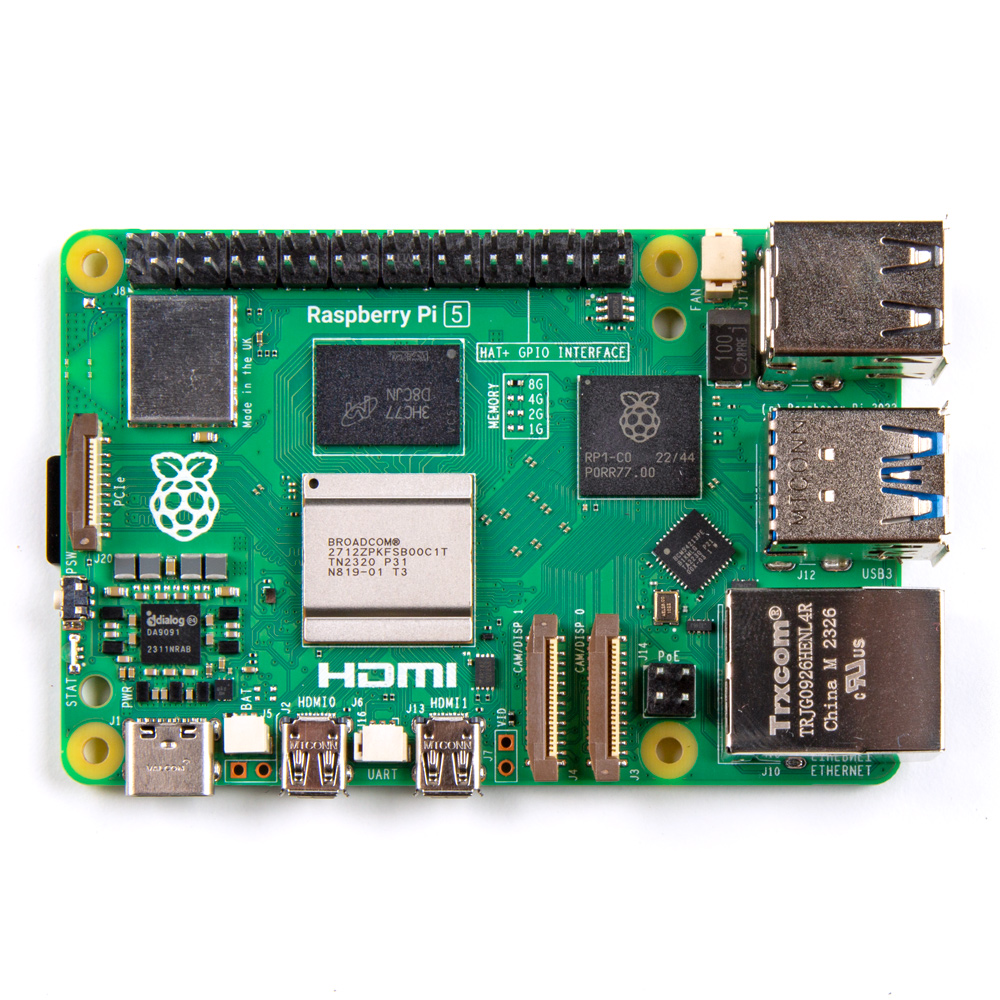
\includegraphics[width=0.6\textwidth]{raspberry-pi-5.jpg}
    \vfill
    {\large \today\par}
\end{titlepage}

\renewcommand{\cftsecleader}{\cftdotfill{\cftdotsep}}

\tableofcontents

\section*{About}  
\addcontentsline{toc}{section}{\protect\numberline{}About}  

This document provides descriptions, instructions and commands for projects using a Raspberry Pi 5. Each project is inspired by a YouTube video, but this document refines and expands upon the content to offer clear guidance for those who wish to replicate the projects. The purpose of collecting this information in a single document is as follows:

\begin{itemize}
\item Some videos lack quality or are no longer relevant. This document selects the useful ones.
\item Some videos do not provide commands in written form. By providing them here, readers can avoid needing to manually retype everything.
\item Some videos could benefit from additional suggestions or improvements. This document expands on those projects to make them more practical.
\end{itemize}

The projects in this document were created using the Raspberry Pi 5 Desktop Kit. However, in most cases, a Raspberry Pi 5 Starter Kit provides all the necessary components to follow along. Additionally, these projects are not specific to the Raspberry Pi 5 as most of them can be completed using other Raspberry Pi models as well.  

In IT, a "project" is defined as a time-bound endeavor with a unique outcome. While this definition does not fully align with how it is used in the document, it remains the closest approximation to describe the work presented here.

\section*{Raspberry Pi 5 preparation}
\addcontentsline{toc}{section}{\protect\numberline{}Raspberry Pi 5 preparation}

Add SSD to the PC using an SSD reader to install an operating system. Use the Raspberry Pi Imager, which is a tool that simplifies the process of installing an operating system onto your Raspberry Pi’s storage device. It has three main options:
\begin{itemize}
\item \textbf{Device}: Select the Raspberry Pi device (in this case, Raspberry Pi 5).
\item \textbf{Operating System}: Choose the OS based on the project requirements. The specific OS used for each project will be specified in the \textbf{Projects Overview} section.
\item \textbf{Storage}: Select the storage device, either a microSD card or an SSD, which will be used to boot and store data for the Raspberry Pi.
\end{itemize}

Raspberry Pi Imager will write the OS to the selected storage and allow you to configure basic settings such as hostname, Wi-Fi, and SSH. Before clicking \textbf{Next}, press \textbf{Ctrl + Shift + X} to customize settings under \textbf{General}, \textbf{Services}, and \textbf{Options}.

For some projects, it may be necessary to connect to the Raspberry Pi remotely. In such cases, you need to determine its IP address and establish a connection by following these steps:

\begin{itemize}  
\item \textbf{Finding the Raspberry Pi's IP Address:} One easy method is using \href{https://www.fing.com/}{\textbf{\color{blue}Fing}}, a network scanning tool available for mobile and desktop. It detects devices on your local network and displays their IP addresses.  
\item \textbf{Accessing the Raspberry Pi via SSH:} You can use \href{https://www.chiark.greenend.org.uk/~sgtatham/putty/}{\textbf{\color{blue}PuTTY}}, a free SSH client for Windows. Open PuTTY, enter the Raspberry Pi's IP address, select \textbf{SSH} as the connection type, and click \textbf{Open}. When prompted, log in using the default credentials.  
\end{itemize}  

Not all projects will require SSH access, but for those that do, these tools help simplify the setup process.  

\section{Hosting a Dark Web Site}

\subsection{Overview}
Video: \href{https://www.youtube.com/watch?v=bllS9tkCkaM}{\textbf{\color{blue}i put a DARK WEB website on a Raspberry Pi!!}} \\
Channel: \href{https://www.youtube.com/@NetworkChuck}{\textbf{\color{blue}NetworkChuck}} \\
Operating System: Raspberry Pi OS (64-bit)

\subsection{Steps}
\begin{enumerate}
    \item Update package lists and install Tor:
    \begin{lstlisting}[language=bash, breaklines=true, breakatwhitespace=true, columns=fullflexible]
    $ sudo apt update
    $ sudo apt install tor
    \end{lstlisting}

   \item Edit the Tor configuration file:
    \begin{lstlisting}[language=bash, breaklines=true, breakatwhitespace=true, columns=fullflexible]
    $ sudo nano /etc/tor/torrc
    \end{lstlisting}
    Uncomment the following lines:
    \begin{lstlisting}[language=bash, breaklines=true, breakatwhitespace=true, columns=fullflexible]
    HiddenServiceDir /var/lib/tor/hidden_service/
    HiddenServicePort 80 127.0.0.1:80
    \end{lstlisting}

    \item Restart the Tor service:
    \begin{lstlisting}[language=bash, breaklines=true, breakatwhitespace=true, columns=fullflexible]
    $ sudo service tor stop
    $ sudo service tor start
    $ sudo service tor status
    \end{lstlisting}

    \item Retrieve your site address:
    \begin{lstlisting}[language=bash, breaklines=true, breakatwhitespace=true, columns=fullflexible]
    $ sudo cat /var/lib/tor/hidden_service/hostname
    \end{lstlisting}

    \item Install and start Nginx:
    \begin{lstlisting}[language=bash, breaklines=true, breakatwhitespace=true, columns=fullflexible]
    $ sudo apt install nginx
    $ sudo service nginx start
    $ sudo service nginx status
    \end{lstlisting}

\item Modify Nginx configuration:
\begin{lstlisting}[language=bash, breaklines=true, breakatwhitespace=true, columns=fullflexible]
$ sudo nano /etc/nginx/nginx.conf
\end{lstlisting}

Uncomment the following lines:
\begin{lstlisting}[language=bash, breaklines=true, breakatwhitespace=true, columns=fullflexible]
port_in_redirect off;
server_name_in_redirect off;
\end{lstlisting}

Add the following line below "port\_in\_redirect off;":
\begin{lstlisting}[language=bash, breaklines=true, breakatwhitespace=true, columns=fullflexible]
server_tokens off;
\end{lstlisting}

    \item Restart Nginx:
    \begin{lstlisting}[language=bash, breaklines=true, breakatwhitespace=true, columns=fullflexible]
    $ sudo service nginx restart
    \end{lstlisting}

    \item Create a simple web page:
    \begin{lstlisting}[language=bash, breaklines=true, breakatwhitespace=true, columns=fullflexible]
    $ cd /var/www/html
    $ sudo rm index.nginx-debian.html
    $ sudo nano index.html
    \end{lstlisting}
    Add your HTML content and save the file.

\item Restart Nginx to apply changes:
\begin{lstlisting}[language=bash, breaklines=true, breakatwhitespace=true, columns=fullflexible]
$ sudo service nginx restart
\end{lstlisting}
Now, your site should be accessible via the generated .onion address!
   
\end{enumerate}

\section{Mining Monero Cryptocurrency}

\subsection{Overview}
Video: \href{https://www.youtube.com/watch?v=hHtGN_JzoP8}{\textbf{\color{blue}How to Mine Monero on Raspberry Pi}} \\
Channel: \href{https://www.youtube.com/@NetworkChuck}{\textbf{\color{blue}NetworkChuck}} \\
Pool: \href{https://moneroocean.stream/}{\textbf{\color{blue}Monero Ocean}} \\
Operating System: Raspberry Pi OS Lite (64-bit)

\subsection{Steps}
\begin{enumerate}
    \item Update package lists and install dependencies:
    \begin{lstlisting}[language=bash, breaklines=true, breakatwhitespace=true, columns=fullflexible]
    $ sudo apt update
    $ sudo apt install git build-essential cmake libuv1-dev libssl-dev libhwloc-dev -y
    \end{lstlisting}

    \item Clone the XMRig repository and build the miner:
    \begin{lstlisting}[language=bash, breaklines=true, breakatwhitespace=true, columns=fullflexible]
    $ git clone https://github.com/xmrig/xmrig.git
    $ cd xmrig
    $ mkdir build
    $ cd build
    $ cmake ..
    $ make
    \end{lstlisting}

    \item Choose one of the following mining options:
    \begin{enumerate}
        \item Standard mining:
        \begin{lstlisting}[language=bash, breaklines=true, breakatwhitespace=true, columns=fullflexible]
        $ ./xmrig -o gulf.moneroocean.stream:10128 -u <YOUR_WALLET_ADDRESS> -p <WORKER_NAME>
        \end{lstlisting}
        
        \item Mining in a detached session using tmux:
        \begin{lstlisting}[language=bash, breaklines=true, breakatwhitespace=true, columns=fullflexible]
        $ tmux
        $ ./xmrig -o gulf.moneroocean.stream:10128 -u <YOUR_WALLET_ADDRESS> -p <WORKER_NAME>
        \end{lstlisting}
        Press \texttt{Ctrl+b}, then \texttt{d} to detach.
        To reattach the session:
        \begin{lstlisting}[language=bash, breaklines=true, breakatwhitespace=true, columns=fullflexible]
        $ tmux attach
        \end{lstlisting}
        
        \item Automating mining with a startup script:
        \begin{lstlisting}[language=bash, breaklines=true, breakatwhitespace=true, columns=fullflexible]
        $ nano start_mining.sh
        \end{lstlisting}
        Add the following lines:
        \begin{lstlisting}[language=bash, breaklines=true, breakatwhitespace=true, columns=fullflexible]
        #!/bin/bash
        cd <BUILD_DIRECTORY_OF_XMRIG>
        tmux new-session -d -s xmrig_session './xmrig -o gulf.moneroocean.stream:10128 -u <YOUR_WALLET_ADDRESS> -p <WORKER_NAME>'
        \end{lstlisting}
        Save and exit, then make the script executable:
        \begin{lstlisting}[language=bash, breaklines=true, breakatwhitespace=true, columns=fullflexible]
        $ chmod +x start_mining.sh
        \end{lstlisting}
        Run the script:
        \begin{lstlisting}[language=bash, breaklines=true, breakatwhitespace=true, columns=fullflexible]
        $ ./start_mining.sh
        \end{lstlisting}
	Now, Monero mining will run in the background, and you can check the session using \texttt{tmux attach}.
    \end{enumerate}
\end{enumerate}

\section{Playing Games with RetroPie}

\subsection{Overview}
Video: \href{https://www.youtube.com/watch?v=AaseHnf0k2o}{\textbf{\color{blue}How to Mine Monero on Raspberry Pi}} \\
Channel: \href{https://www.youtube.com/@NetworkChuck}{\textbf{\color{blue}NetworkChuck}} \\
Operating System: Raspberry Pi OS Lite (64-bit)

\subsection{Steps}

\begin{enumerate}
    \item Update and upgrade packages:
    \begin{lstlisting}[language=bash, breaklines=true, breakatwhitespace=true, columns=fullflexible]
    $ sudo apt update
    $ sudo apt upgrade -y
    $ sudo apt install git lsb-release
    \end{lstlisting}

   \item Clone the RetroPie setup script:
    \begin{lstlisting}[language=bash, breaklines=true, breakatwhitespace=true, columns=fullflexible]
    $ cd
    $ git clone https://github.com/retropie/retropie-setup.git
    $ cd retropie-setup
    $ chmod +x retropie_setup.sh
    \end{lstlisting}

    \item Run the setup script:
    \begin{lstlisting}[language=bash, breaklines=true, breakatwhitespace=true, columns=fullflexible]
    $ sudo ./retropie_setup.sh
    \end{lstlisting}
    Navigate through the setup: OK → OK → Basic install → Yes. The installation process will take a while. After completion, navigate to Configuration/Tools → Autostart → OK → bashwelcometweak → OK → Exit.

    \item Reboot the system:
    \begin{lstlisting}[language=bash, breaklines=true, breakatwhitespace=true, columns=fullflexible]
    $ sudo reboot
    \end{lstlisting}

    \item Transfer ROMs to RetroPie:
    ROMs can be downloaded from \href{https://www.emulatorgames.net}{\textbf{\color{blue}emulatorgames.net}} and \href{https://www.romsgames.net}{\textbf{\color{blue}romsgames.net}}. Use SCP to transfer ROMs from your desktop:
    \begin{lstlisting}[language=bash, breaklines=true, breakatwhitespace=true, columns=fullflexible]
    $ scp -r ~/Desktop/roms/* username@<YOUR_IP>:~/RetroPie/roms/
    \end{lstlisting}

    \item Configure Raspberry Pi settings in RASPI-CONFIG:
    \begin{itemize}
        \item System Options → Set Hostname, Change Password
        \item Localisation Options → Set Timezone, WLAN Country
        \item Interface Options → Enable SSH
    \end{itemize}

    \item Connect to WiFi (outside RASPI-CONFIG) and restart.

    \item Entering and exiting EmulationStation:
    Pressing \textbf{F4} will take you to the command line interface (CLI). To return to EmulationStation, enter:
    \begin{lstlisting}[language=bash, breaklines=true, breakatwhitespace=true, columns=fullflexible]
    $ emulationstation
    \end{lstlisting}
    ROMs must be placed in their respective emulator directories, e.g., \texttt{~/RetroPie/roms/psx} for PlayStation games.
    
    \item Reference supported systems at \href{https://retropie.org.uk/docs/Supported-Systems/}{\textbf{\color{blue}RetroPie Supported Systems}}.
    
    \item Configure input mappings for controllers.
    
    \item Set up hotkeys:
    \begin{itemize}
        \item \textbf{HOTKEY + Start}: Exit game
        \item \textbf{HOTKEY + Right Shoulder}: Save game
        \item \textbf{HOTKEY + Left Shoulder}: Load game
        \item \textbf{HOTKEY + D-PAD Right}: Change save/load slot
        \item \textbf{HOTKEY + Button B}: Reset game
        \item \textbf{HOTKEY + Button X}: Open RetroArch menu
    \end{itemize}
    
    \item Personalize game lists:
    \begin{itemize}
        \item UI Settings → Set Game List View Style to Grid
        \item Scraper → Scrape from ScreenScraper → Scrape Now
    \end{itemize}
    
    \item Enable cheats:
    \begin{enumerate}
        \item Open RetroArch menu (HOTKEY + Button X)
        \item Enable Advanced Settings
        \item Update Cheats via Online Updater
        \item Load Cheat File and apply changes
    \end{enumerate}

    \item Enable achievements:
    \begin{enumerate}
        \item Register at \href{https://retroachievements.org}{\textbf{\color{blue}RetroAchievements}}
        \item Configure username and password in RetroArch Settings
        \item Save configuration and restart
    \end{enumerate}
\end{enumerate}

\section{Setting Up a NAS with Samba}

\subsection{Overview}
Video: \href{https://www.youtube.com/watch?v=8QxJWW0mjAs}{\textbf{\color{blue}Pi Network File Share to Windows \& More | Pi NAS/SMB | Raspberry Pi Guide}} \\
Channel: \href{https://www.youtube.com/@TroubleChute}{\textbf{\color{blue}TroubleChute}} \\
Operating System: Raspberry Pi OS Lite (64-bit)

A NAS (Network-Attached Storage) is a device that allows file sharing over a network. In this guide, we will set up Samba on a Raspberry Pi, enabling file sharing using the SMB (Server Message Block) protocol. This will allow different devices to access shared files on the Raspberry Pi.

\subsection{Steps}
\begin{enumerate}
    \item Update your system and install Samba:
    \begin{lstlisting}[language=bash, breaklines=true, breakatwhitespace=true, columns=fullflexible]
    $ sudo apt update && sudo apt upgrade
    $ sudo apt install samba samba-common-bin
    \end{lstlisting}

    \item Create a shared directory:
    \begin{lstlisting}[language=bash, breaklines=true, breakatwhitespace=true, columns=fullflexible]
    $ mkdir ~/shared
    \end{lstlisting}

    \item Edit the Samba configuration file:
    \begin{lstlisting}[language=bash, breaklines=true, breakatwhitespace=true, columns=fullflexible]
    $ sudo nano /etc/samba/smb.conf
    \end{lstlisting}
    Add the following at the end of the file:
    \begin{lstlisting}[language=bash, breaklines=true, breakatwhitespace=true, columns=fullflexible]
    [shared]
    path=/home/<USERNAME>/shared
    writable=Yes
    create mask=0666
    directory mask=0666
    public=no
    \end{lstlisting}

    \item Set a Samba password for your user:
    \begin{lstlisting}[language=bash, breaklines=true, breakatwhitespace=true, columns=fullflexible]
    $ sudo smbpasswd -a <USERNAME>
    \end{lstlisting}

    \item Restart the Samba service:
    \begin{lstlisting}[language=bash, breaklines=true, breakatwhitespace=true, columns=fullflexible]
    $ sudo systemctl restart smbd
    \end{lstlisting}

    \item Find your Raspberry Pi's IP address:
    \begin{lstlisting}[language=bash, breaklines=true, breakatwhitespace=true, columns=fullflexible]
    $ hostname -I
    \end{lstlisting}

    \item To access the shared directory from a Windows computer, follow these steps:
     \begin{enumerate}
        \item Open \textit{This PC}.
        \item Right-click on the empty space and select \textit{Add a network location}.
        \item Follow the prompts: Click \textit{Next}, then \textit{Next} again.
        \item Enter the network path in the format: \texttt{\\*Add ip*/shared} and click \textit{Next}.
      \end{enumerate}

\end{enumerate}

\section{Running Large Language Models (LLMs) on Raspberry Pi 5 with Ollama}

\subsection{Overview}
Video: \href{https://www.youtube.com/watch?v=nNxtQhz1b2M}{\textbf{\color{blue}Raspberry Pi 5 AI Setup Guide: Run DeepSeek, TinyLlama +more LOCALLY!}} \\
Channel: \href{https://www.youtube.com/@WagnersTechTalk}{\textbf{\color{blue}Wagner's TechTalk}} \\
Operating System: Raspberry Pi OS Lite (64-bit)

\subsection{Steps}
\begin{enumerate}
    \item Update your Raspberry Pi:
    \begin{lstlisting}[language=bash, breaklines=true, breakatwhitespace=true, columns=fullflexible]
    $ sudo apt update
    $ sudo apt upgrade
    \end{lstlisting}

    \item Install Ollama:
    \begin{lstlisting}[language=bash, breaklines=true, breakatwhitespace=true, columns=fullflexible]
    $ curl -fsSL https://ollama.com/install.sh | sh
    \end{lstlisting}
    After installation, verify the version of Ollama installed:
    \begin{lstlisting}[language=bash, breaklines=true, breakatwhitespace=true, columns=fullflexible]
    $ ollama -v
    \end{lstlisting}

    \item Run the LLM:

    To run TinyLlama (1.1 billion parameters / 637MB):
    \begin{lstlisting}[language=bash, breaklines=true, breakatwhitespace=true, columns=fullflexible]
    $ ollama run tinyllama
    \end{lstlisting}

    To run DeepSeek-R1 (1.5 billion parameters / 1.1GB):
    \begin{lstlisting}[language=bash, breaklines=true, breakatwhitespace=true, columns=fullflexible]
    $ ollama run deepseek-r1:1.5b
    \end{lstlisting}

    The first time you run a new LLM, it will download the model, so it will take longer. 	

    \item Ask the LLM a question by typing any question and pressing \texttt{ENTER}. Keep in mind that running an LLM on the Raspberry Pi 5 may be slower than using an online platform.
    
    \item Ollama LLM Commands:

    \begin{itemize}
        \item \texttt{/set} – Set session variables
        \item \texttt{/show} – Show model information
        \item \texttt{/load <model>} – Load a session or model
        \item \texttt{/save <model>} – Save your current session
        \item \texttt{/clear} – Clear session context
        \item \texttt{/bye} – Exit the LLM
        \item \texttt{/?}, \texttt{/help} – Help for a command
        \item \texttt{/? shortcuts} – Help for keyboard shortcuts
    \end{itemize}

    \item Exit Ollama:
    \begin{lstlisting}[language=bash, breaklines=true, breakatwhitespace=true, columns=fullflexible]
    $ /bye
    \end{lstlisting}
    or press \texttt{Ctrl+D}.

    \item List Installed Models:
    \begin{lstlisting}[language=bash, breaklines=true, breakatwhitespace=true, columns=fullflexible]
    $ ollama list
    \end{lstlisting}

    \item Remove a Model:
    \begin{lstlisting}[language=bash, breaklines=true, breakatwhitespace=true, columns=fullflexible]
    $ ollama rm <model>
    \end{lstlisting}
    Example for removing DeepSeek-R1:
    \begin{lstlisting}[language=bash, breaklines=true, breakatwhitespace=true, columns=fullflexible]
    $ ollama rm deepseek-r1:1.5b
    \end{lstlisting}

    \item Remove Ollama:
    \begin{lstlisting}[language=bash, breaklines=true, breakatwhitespace=true, columns=fullflexible]
    $ sudo systemctl stop ollama
    $ sudo systemctl disable ollama
    $ sudo rm /etc/systemd/system/ollama.service
    \end{lstlisting}

\end{enumerate}

\subsection{Additional Resources}
Many other models can be found on the official Ollama website: \href{https://ollama.com/search}{\textbf{\color{blue}Ollama Model Search}}.

\section{Setting Up Pi-hole for Network-wide Ad Blocking}

\subsection{Overview}
Video: \href{https://www.youtube.com/watch?v=cE21YjuaB6o}{\textbf{\color{blue}World's Greatest Pi-hole Tutorial - Easy Raspberry Pi Project!}} \\
Channel: \href{https://www.youtube.com/@CrosstalkSolutions}{\textbf{\color{blue}Crosstalk Solutions}} \\
Operating System: Raspberry Pi OS Lite (64-bit)

Pi-hole is a network-wide ad blocker that acts as a DNS sinkhole, filtering out advertisements before they reach your devices. This guide will walk you through setting up Pi-hole on a Raspberry Pi and configuring your network to use it as the primary DNS server.

\subsection{Steps}
\begin{enumerate}
    \item Update your system:
    \begin{lstlisting}[language=bash, breaklines=true, breakatwhitespace=true, columns=fullflexible]
    $ sudo apt update && sudo apt upgrade -y
    \end{lstlisting}

    \item Install the DHCP client daemon (needed for a static IP setup):
    \begin{lstlisting}[language=bash, breaklines=true, breakatwhitespace=true, columns=fullflexible]
    $ sudo apt install dhcpcd
    \end{lstlisting}
    
    \item Configure a static IP address:
    \begin{lstlisting}[language=bash, breaklines=true, breakatwhitespace=true, columns=fullflexible]
    $ sudo nano /etc/dhcpcd.conf
    \end{lstlisting}

    Add the following lines at the end of the file:
    \begin{lstlisting}[language=bash, breaklines=true, breakatwhitespace=true, columns=fullflexible]
    interface wlan0
    static ip_address=<YOUR_IP>/24
    static routers=<YOUR_ROUTER_IP>
    static domain_name_servers=<DNS_SERVER_1> <DNS_SERVER_2>
    \end{lstlisting}

    Save the file and reboot the Raspberry Pi:
    \begin{lstlisting}[language=bash, breaklines=true, breakatwhitespace=true, columns=fullflexible]
    $ sudo reboot
    \end{lstlisting}

    \item Install Pi-hole using the automated script:
    \begin{lstlisting}[language=bash, breaklines=true, breakatwhitespace=true, columns=fullflexible]
    $ curl -sSL https://install.pi-hole.net | bash
    \end{lstlisting}

    Follow the installation prompts:
    \begin{itemize}
        \item \textbf{Pi-hole Automated Installer:} Select OK
        \item \textbf{Open Source Software:} Select OK
        \item \textbf{Static IP Needed:} Select Continue
        \item \textbf{Choose An Interface:} Select wlan0
        \item \textbf{Select Upstream DNS Provider:} Choose Google (or another preferred provider)
        \item \textbf{Blocklists:} Select Yes
        \item \textbf{Enable Logging:} Select Yes
        \item \textbf{Select a privacy mode for FTL:} Choose "Show everything"
        \item \textbf{Installation Complete:} Select OK
    \end{itemize}

    \item Access the Pi-hole web interface:
    \begin{lstlisting}[language=bash, breaklines=true, breakatwhitespace=true, columns=fullflexible]
    https://<YOUR_IP>/admin
    \end{lstlisting}

    \item Configure devices to use Pi-hole manually (Example for Windows):
    \begin{enumerate}
        \item Open \textit{Network Connections}.
        \item Right-click on your Wi-Fi connection and select \textit{Properties}.
        \item Select \textit{Internet Protocol Version 4 (TCP/IPv4)} and click \textit{Properties}.
        \item Choose \textit{Use the following DNS server addresses} and enter:
        \begin{itemize}
            \item Preferred DNS server: \texttt{\textless YOUR\_IP\textgreater}
            \item Alternate DNS server: Leave blank or use another DNS (e.g., 1.1.1.1)
        \end{itemize}
        \item Click OK to apply changes.
    \end{enumerate}

    \item Ensure Raspberry Pi uses Pi-hole for its own DNS queries:
    \begin{lstlisting}[language=bash, breaklines=true, breakatwhitespace=true, columns=fullflexible]
    $ sudo nano /etc/resolv.conf
    \end{lstlisting}

    Replace the contents with:
    \begin{lstlisting}[language=bash, breaklines=true, breakatwhitespace=true, columns=fullflexible]
    nameserver <YOUR_IP>
    \end{lstlisting}

    Lock the file to prevent modifications:
    \begin{lstlisting}[language=bash, breaklines=true, breakatwhitespace=true, columns=fullflexible]
    $ sudo chattr +i /etc/resolv.conf
    \end{lstlisting}
 
    (To unlock the file for changes, use: \texttt{\$ sudo chattr -i /etc/resolv.conf})

    \item Reboot the Raspberry Pi to apply changes:
    \begin{lstlisting}[language=bash, breaklines=true, breakatwhitespace=true, columns=fullflexible]
    $ sudo reboot
    \end{lstlisting}

\end{enumerate}

\end{document}
